\chapter{Kravspecifikation (Alle)}

\section{Version}
\begin{table}[h]
	\centering
	\begin{tabularx}{\textwidth - 2cm}{|l|l|l|X|}
	\hline
	Dato	& Version	& Initialer & Ændring	\\ \hline
	26. februar & 1 & MHG & Første udkast. \\ \hline
	6. marts & 2 & MHG & Rettelser efter review. \\ \hline
	\end{tabularx}
\end{table}

\section{Systembeskrivelse}

Systemet AutoGreen fungerer som et intelligent drivhus, med hovedformålene at kunne monitorere og regulere nogle forskellige parametre i drivhusets indre. Blandt parametrene vil der være jordfugt-, luftfugt-, temperatur- og lyssensorer og de enheder, som systemet kommer til at bestå af, kan ses på Figur \ref{fig:systemoversigt}. Nogle af parametrene vil desuden kunne reguleres, således det bliver muligt for en bruger at kunne automatisere sit drivhus. Selve drivhuset som projektet drejer sig om, er en mindre model, med dimensioner som set på Figur \ref{fig:dimensioner}. 

\begin{figure}[!h]
\centering 
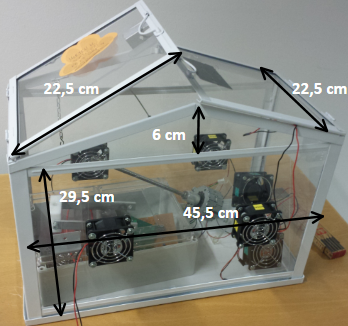
\includegraphics[scale=0.9] {../fig/dimensioner.png}
\caption{Dimensioner for drivhus.}
\label{fig:dimensioner}
\end{figure}

Ud fra billedet ses blæsere samt vinduesmotoren (ej monteret på billedet), som skal regulere temperaturen i drivhuset. Disse indgår som en del af systemet, men selve huset gør ikke. Der vil ydermere være et varmelegeme, som ikke er repræsenteret på billedet. 

\subsubsection{DevKit8000}
DevKit8000 er systemets kontrolenhed og brugergrænseflade. 
DevKit8000 modtager input fra brugeren på dens touch skærm, og den kan give output til brugeren på skærmen og via e-mail; den er koblet til internet via ethernet. 
DevKit8000 kan desuden måle og regulere klimaet i det fysiske drivhus; det sker vha. en \IIC Master, hvortil der kommunikeres vha. UART.
\subsubsection{\IIC Master}
I\textsuperscript{2}C Master er realiseret på et PSoC4 udviklingsboard (CY8CKIT-042). 
\IIC Master modtager input fra DevKit8000 og sender/modtager data til/fra \IIC Slaver, hvorefter respons sendes retur til DevKit8000.	
\subsubsection{\IIC Slave Temperatur}
\IIC Slave Temperatur er ansvarlig for alle handlinger og målinger, der har med temperaturen i det fysiske drivhus at gøre. Der er tilkoblet en temperatursensor og tre aktuatorer, hhv. vinduesåbner, blæsere og varmelegeme. 
Enheden er realiseret på et PSoC4 udviklingsboard (CY8CKIT-042).
\subsubsection{\IIC Slave Jordfugtighed}
\IIC Slave Jordfugtighed er ansvarlig for alle handlinger og målinger, der har at gøre med vanding i det fysiske drivhus. Der kan tilkobles 0 - 6 jordfugtighedssensorer med tilhørende aktuator til et evt. vandingssystem. Selve vandingssystemet er ikke en del af AutoGreen, en vandingsaktuator er en high/low bool. Enheden er realiseret på et PSoC4 udviklingsboard (CY8CKIT-042).
\subsubsection{\IIC Slave Luftfugtighed/Lys}
\IIC Slave Luftfugtighed/Lys er ansvarlig for måling af lysintensitet og luftfugtighed i det fysiske drivhus. Enheden er realiseret på et PSoC4 udviklingsboard (CY8CKIT-042).

\clearpage

\begin{figure}[!h]
\centering 
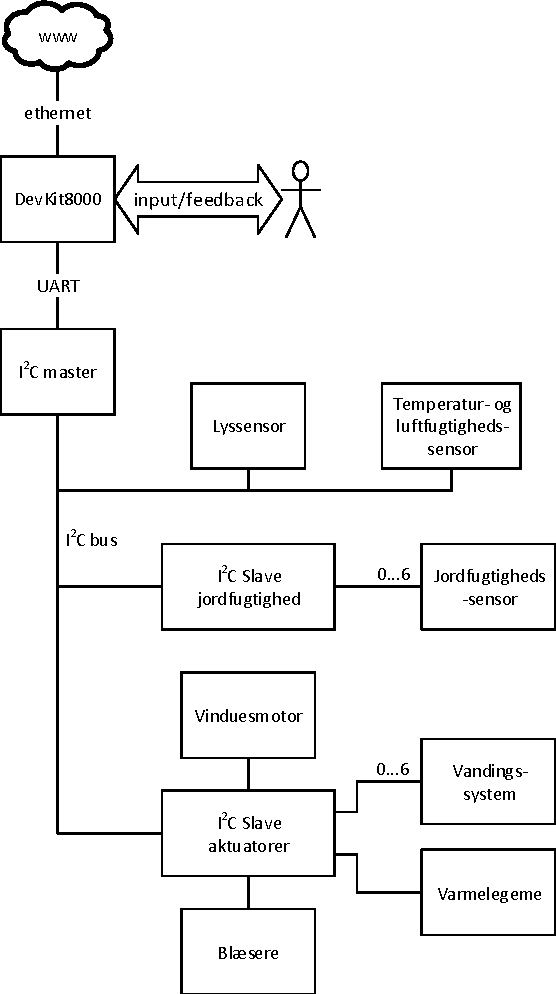
\includegraphics[height={\textheight - 2 cm}, trim=0 0 0 0, clip=true] {../fig/systemoversigt/sys_fig.pdf}
\caption{Oversigt over system}
\label{fig:systemoversigt}
\end{figure}

\clearpage

\section{Ordforklaring}

\subsubsection{Plantedatabase}
Plantedatabasen indeholder information om ideelle forhold for forskellige typer planter, som brugeren kunne tænkes at plante i sit fysiske drivhus. 
Informationen i plantedatabasen står til grund for udgangsparametre for nye planter i det virtuelle drivhus. Der findes en række systemplanter, som brugeren ikke kan redigere eller slette, men brugeren kan tilføje egne planter.
\subsubsection{Data Log}
Systemet er udstyret med en log over de indsamlede data fra sensorer i systemet, der måles og indskrives i loggen hvert minut. 
Denne er opbygget som en database, hvor hver logning indeholder information fra de diskrete sensorer samt et tidspunkt. 
\subsubsection{System Log}
Systemet er udstyret med en log over hvad systemet foretager sig. 
Dette kunne f.eks. være et indlæg når systemet foretager en måling, sender en e-mail, regulerer miljøet i drivhuset.
\subsubsection{Virtuelt Drivhus}
Det virtuelle drivhus er oversigten over planter samt information omkring miljø, som brugeren kan se i selve systemet. 
\subsubsection{Fysisk Drivhus}
Ved det fysiske drivhus forstås det drivhus hvori systemet er monteret. 
Det virtuelle drivhus skal så vidt muligt afspejle det fysiske drivhus, hvor brugeren har sine planter.
\subsubsection{Konfigurationsfil}
Dette er en automatisk genereret fil, der er placeret på dev-kittet, som indeholder brugerens konfigurationer om blandt andet notifikationer, e-mailadresser, antallet af fugtsensorer og deres unikke id mm.

\clearpage

\section{Brugerfladen}

I Figur \ref{fig:gui_skitse} er vist en skitse over hvordan brugerfladen forventes at se ud. De grå områder uner Hovedmenu er knapper, brugeren kan trykke på for at tilgå yderligere menuer. Nederst ses "Monitorer" og "Reguler" knapper, som kan aktivere eller deaktivere hhv. monitorerings- og reguleringsfunktionalitet. Til højre ses live status for det fysiske drivhus, samt live status for jordfugtighed for hver plante i bunden. I bunden af billedet til højre, kan der ses nogle knapper i forskellige farver. Disse symboliserer planter i det virtuelle drivhus, og forklarer tilfældet for den enkelte plante. Grøn betyder at plantens jordfugtighed er indenfor tolerancerne, hvor rød betyder det modsatte. Grå (Not Available) betyder at der ikke er placeret en plante i det virtuelle drivhus, for den pågældende fugtighedssensor. 

\begin{figure}[h]
\centering
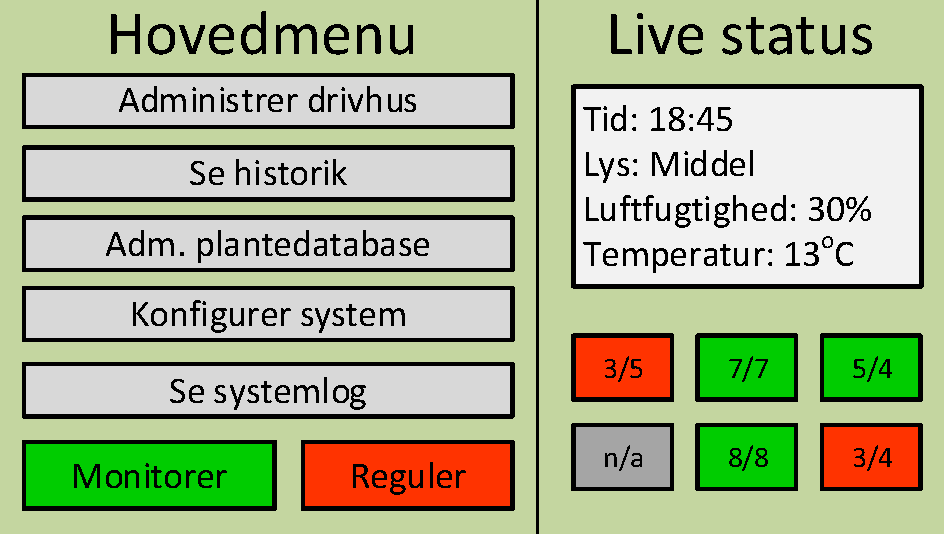
\includegraphics[width=\textwidth - 3 cm]{../fig/gui_skitse}
\caption{Skitse af hovedmenuen på brugerfladen.}
\label{fig:gui_skitse}
\end{figure}

\clearpage

\section{Aktør Kontekst Diagram} 
\begin{figure}[h]
\centering 
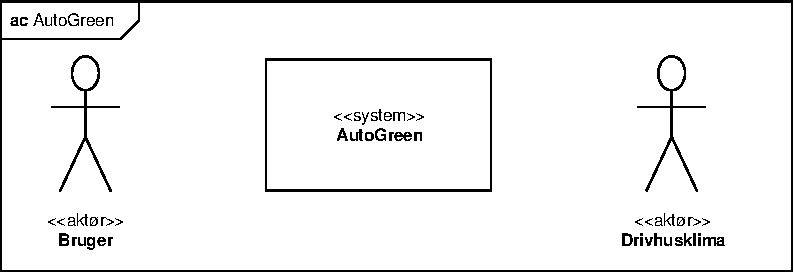
\includegraphics[width={\textwidth}, trim=0 0 0 0, clip=true] {../fig/Aktoer_Kontekst_Diagram.pdf}
\caption{Aktør Kontekst Diagram for AutoGreen}
\label{fig:aktoer_kontekst_diagram}
\end{figure}

\subsection{Aktørbeskrivelser}

\subsubsection{Bruger - Primær Aktør}
Brugeren kan:
\begin{itemize}
\item Starte og stoppe systemet 
\item Overvåge det aktuelle klima i drivhuset. 
\item Administrere drivhuset, hvilket vil sige at han giver systemet input om hvilke planter der er i drivhuset. 
\item Se historik over klimaet i drivhuset
\item Konfigurere systemindstillinger
\item Se systemlog
\item Modtage rapportering om klimaet i drivhuset 
\end{itemize}

\subsubsection{Drivhusklima - Sekundær Aktør}
Drivhusklimaet består af en række parametre, som systemet måler og/eller regulerer:
\begin{itemize}
\item Lufttemperatur
	\subitem Måles, registreres og reguleres af systemet
\item Jordfugtighed
	\subitem Måles, registreres og reguleres indirekte af systemet
\item Luftfugtighed
	\subitem Måles og registreres af systemet
\item Lysintensitet
	\subitem Måles og registreres af systemet
\end{itemize}

\section{Funktionelle Krav}
Systemet\ldots
\begin{enumerate}\itemsep1pt \parskip0pt \parsep0pt
	\item \ldots \emph{Skal} give brugeren mulighed for at monitorere og konfigurere drivhusklimaet vha. en grafisk brugerflade på et touch display.
	\item \ldots \emph{Skal} have mulighed for at starte og stoppe systemet.
	\item \ldots \emph{Skal} måle lufttemperatur i det fysiske drivhus.
	\item \ldots \emph{Skal} kunne regulere temperatur i det fysiske drivhus.
	\item \ldots \emph{Skal} kunne indstilles til brugerdefineret tid og dato.
	\item \ldots \emph{Skal} kunne give brugeren mulighed for at vælge brug af varmelegeme og ventilatorer.
	\item \ldots \emph{Skal} give brugeren mulighed for at tilføje en plante i det virtuelle drivhus.
	\item \ldots \emph{Skal} give brugeren mulighed for at fjerne en plante i det virtuelle drivhus.
	\item \ldots \emph{Skal} give brugeren mulighed for at redigere en plante i det virtuelle drivhus.
	\item \ldots \emph{Skal} kunne regulere drivhusklima automatisk efter behov.
	\item \ldots \emph{Bør} kunne måle jordfugtighed i fysiske drivhus.
	\item \ldots \emph{Bør} kunne måle lysintensitet i det fysiske drivhus.
	\item \ldots \emph{Bør} kunne måle luftfugtighed i det fysiske drivhus.
	\item \ldots \emph{Bør} indeholde informationer om planter i en datastruktur.
	\item \ldots \emph{Bør} kunne fremvise grafisk historik over måledata fra drivhus.
	\item \ldots \emph{Bør} kunne vise planteinformationer fra plantedatabasen.
	\item \ldots \emph{Bør} give brugeren mulighed for at se en systemlog over hændelser i systemet.
	\item \ldots \emph{Bør} gemme alt monitorering i en data log.
	\item \ldots \emph{Kan} give brugeren mulighed for at redigere og slette planter i plantedatabasen, som brugeren selv har tilføjet.
	\item \ldots \emph{Kan} give brugeren mulighed for at tilføje/redigere/slette e-mail adresser.
	\item \ldots \emph{Kan} give brugeren mulighed for valg af varslingse-mail omhandlende dårligt klima og daglig e-mail.
	\item \ldots \emph{Kan} sende e-mail til brugeren, på baggrund af brugerindstillinger.
\end{enumerate}

\section{Ikke Funktionelle Krav}
Systemet\ldots
\begin{enumerate}\itemsep1pt \parskip0pt \parsep0pt
	\item \ldots \emph{Skal} minimum måle parametre i det fysiske drivhus med 1 minuts mellemrum +/- 5 sekunder.
	\item \ldots \emph{Skal} kunne justere temperaturen i det fysiske drivhus til det ønskede niveau på højst 30 minutter ved en starttemperatur der ligger højst 10 grader fra det ønskede niveau, når alle tre aktuatorer anvendes.
	\item \ldots \emph{Skal} kunne måle jordfugtighed i trin á 10, hvor 10 er mest fugtigt. 
	\item \ldots \emph{Skal} kunne indeholde op til seks fugtmålere.
	\item \ldots \emph{Skal} anvende DevKit8000 med indlejret Linux platform.
	\item \ldots \emph{Skal} anvende mindst et PSOC 4 udviklingsboard.
	\item \ldots \emph{Skal} kunne indeholde op til 100 planter i plantedatabasen.
	\item \ldots \emph{Skal} kunne indeholde data et år tilbage i tiden.
	\item \ldots \emph{Skal} kunne måle temperaturen med en præcision på +/- 1 grad celcius ved 20 grader.
	\item \ldots \emph{Skal} kunne indeholde op til tre e-mail adresser.
	\item \ldots \emph{Bør} kunne justere temperaturen til 25 grader celcius i det fysiske drivhus med en præcision på +/- 2 grad, når drivhuset er placeret i et rum ved stuetemperatur (ca. 20 grader).
	\item \ldots \emph{Kan} sende mail til brugeren højest 1 minut efter et for lavt jordfugtighedsniveau er målt, hvis den er indstillet til dette.
\end{enumerate}


\section{Use Case Diagram}
\begin{figure}[h]
\centering 
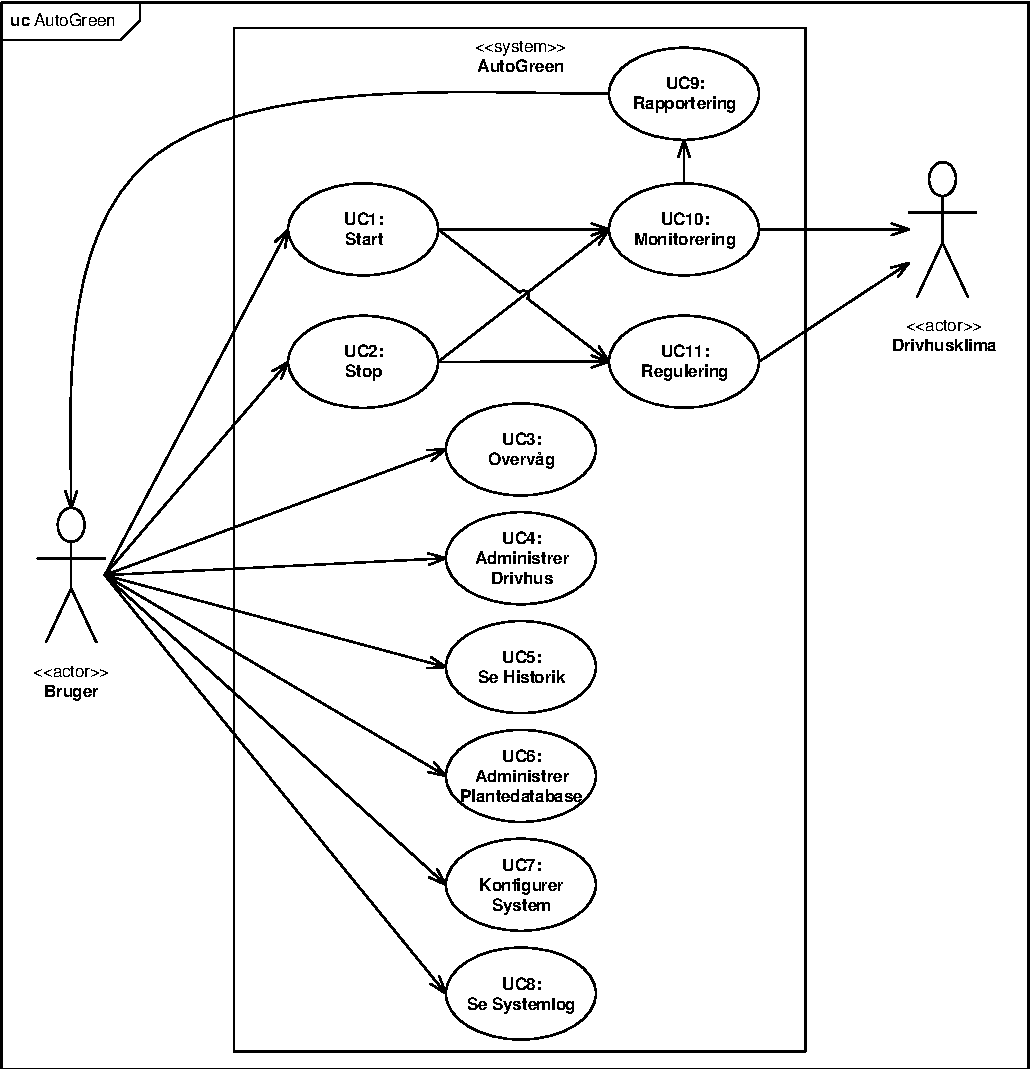
\includegraphics[width={\textwidth-1cm}, trim=0 0 0 0, clip=true] {../fig/UC_Diagram.pdf}
\caption{Use Case Diagram for AutoGreen}
\label{fig:use_case_diagram}
\end{figure}

\clearpage

\subsection{Use Case beskrivelser - Initiering og Formål}
\subsubsection{UC1: Start}
Initieres af: Bruger

Denne UC giver brugeren mulighed for at starte systemet, dvs. monitorering og regulering af drivhusklimaet. 
Brugeren har mulighed for kun at starte monitorering. Use Case’en kan initiere UC10 Rapportering og UC11 Monitorering.

\subsubsection{UC2: Stop}
Initieres af: Bruger

Denne UC giver brugeren mulighed for at stoppe systemet, dvs. monitorering og regulering af drivhusklimaet. 
Brugeren har mulighed for kun at stoppe regulering. Use Case’en kan stoppe UC10 Rapportering og UC11 Monitorering.

\subsubsection{UC3: Overvåg}
Initieres af: Bruger

Når monitorering er startet, vises der i user interfacets hovedmenu live opdaterede måleværdier. 
Såfremt UC10 Monitorering er startet, kan værdierne for lufttemperatur og jordfugtighed være røde, hvis de ikke passer med de ønskede værdier.

\subsubsection{UC4: Administrer Drivhus}
Initieres af: Bruger

Denne UC giver brugeren mulighed for at informere systemet om hvilke planter der er i drivhuset. 
Han kan tilføje op til seks planter fra plantedatabasen i drivhuset, og han kan redigere parametre for disse, hvis han ønsker andre parametre end dem der fremgår i plantedatabasen. 
Hver af disse planter kan forbindes med en jordfugtighedsmåler. 

\subsubsection{UC5: Se Historik}
Initieres af: Bruger

Denne Use Case giver brugeren mulighed for at se grafisk historik over de fire målte parametre i drivhuset. 
Brugeren kan se data op til et år tilbage i tiden. 

\subsubsection{UC6: Administrer Plantedatabase}
Initieres af: Bruger

Denne UC giver brugeren mulighed for at se på planter i databasen. 
Han kan desuden tilføje og fjerne egne planter i databasen, og han kan redigere i de planter han tidligere har tilføjet. 
Han kan ikke redigere eller fjerne planter han ikke selv har tilføjet. 

\subsubsection{UC7: Konfigurer System}
Initieres af: Bruger

Denne UC giver brugeren mulighed for at rette i systemindstillinger, herunder:
\begin{itemize}
\item Indstille tid og dato
\item Tilføje/fjerne/rette e-mail adresse 
\item Aktivering/deaktivering af advarsler om dårligt klima sendt pr. mail
\item Aktivering/deaktivering af daglig status sendt pr. mail
\item Aktivering/deaktivering af varmelegeme
\item Aktivering/deakttivering af luftcirkulation
\end{itemize}

\subsubsection{UC8: Se System Log}
Initieres af: Bruger/Tekniker

Denne UC giver brugere eller teknikeren mulighed for at se en liste over systemhændelser, herunder:
\begin{itemize}
\item Start og stop af system
\item Manglende kontakt til sensorer
\item Afsendte e-mails
\item Tilføjede/fjernede/redigerede planter i drivhuset
\item Tilføjede/fjernede/redigerede planter i plantedatabasen
\item Konfigurationsændringer
\item Fejl i registrering i datalog
\item Fejl på vinduesåbner
\item Fejl på Luftcirkulation
\item Fejl på varmelegeme
\end{itemize}

\subsubsection{UC9: Rapportering}
Initieres af: UC10 Monitorering

Denne Use Case rapporterer til brugeren ud fra de indstillinger brugeren har valgt under UC7 Konfigurer System. 
Dette sker ved afsendelse af e-mail til den eller de adresser, som brugeren ligeledes har tilføjet under UC7 Konfigurer System.

\subsubsection{UC10: Monitorering}
Initieres af: UC1 Start.

Denne Use Case lagrer kontinuerligt målinger af lufttemperatur, jordfugtighed, luftfugtighed og lysintensitet i en data log fil. 
Lagringen sker en gang i minuttet. 

\subsubsection{UC11: Regulering}
Initeres af: UC1 Start.

Denne Use Case regulerer temperaturen i drivhuset, som udgangspunkt vha. vinduesåbner, varmelegeme og luftcirkulation. 
Det kan ske uden luftcirkulation og/eller varmelegeme, hvis brugeren har valgt dette under UC7 Konfigurer System. Det er ikke muligt at aktivere regulering uden at UC10 Monitorering er aktiveret.

\clearpage

\subsection{Use Case Beskrivelser - Fully Dressed}
For alle Use Cases hvor brugeren navigerer i undermenuer af hovedmenuen, gælder det, at brugeren har mulighed for at gå et skridt tilbage ved at trykke på en ”tilbage knap”. Fremover ved benævningen ”Systemet er operationelt” menes, at systemet er tilsluttet tilstrækkelig strømforsyning og at alt fungerer efter hensigten og at systemet er tilsluttet ethernet.

%UC1
\begin{table}[h]
\begin{tabularx}{\textwidth}{| >{\raggedright\arraybackslash}p{3.3 cm} | >{\raggedright\arraybackslash}X |} \hline

\textbf{Navn:} 						& UC1: Start\\ \hline
\textbf{Mål:}						& At starte systemet helt eller delvist. \\ \hline
\textbf{Initering:}					& Bruger \\ \hline
\textbf{Aktører:} 					& Bruger (primær) \\ \hline
\textbf{Reference:} 					& UC10: Monitorering, UC11: Regulering \\ \hline
\textbf{Antal samtidige forekomster:} & En \\ \hline
\textbf{Forudsætning:} 				& Systemet er stoppet helt, er operationelt og viser hovedmenuen.\\ \hline
\textbf{Resultat:}					& At systemet er startet helt eller delvist. \\ \hline
\textbf{Hovedscenarie:}				& 

\begin{packed_enum}
\item Bruger trykker på monitorerings knap. 
\item System aktiverer UC10: Monitorering. 
\item Bruger trykker på regulerings knap. 
	\begin{packed_item}\itemsep1pt \parskip0pt \parsep0pt
	\item {[}Ext 3.a : Bruger vælger kun monitorering.{]}
	\end{packed_item}
\item Systemet aktiverer UC11: Regulering.
\end{packed_enum} \\ \hline
\textbf{Udvidelser:}				&  
\textbf{{[}Ext 3.a : Bruger vælger kun monitorering.{]}}
	\begin{packed_enum}\itemsep1pt \parskip0pt \parsep0pt
	\item Systemet fortsætter ved pkt. 5 i hovedscenarie.
	\end{packed_enum}
\\ \hline
\end{tabularx}
\caption{UC1: Start}
\label{tbl:UC1}
\end{table}

\clearpage
%UC2
\begin{table}[h]
\begin{tabularx}{\textwidth}{| >{\raggedright\arraybackslash}p{3.3 cm} | >{\raggedright\arraybackslash}X |} \hline

\textbf{Navn:} 						& UC2: Stop\\ \hline
\textbf{Mål:}						& At stoppe systemet helt eller delvist. \\ \hline
\textbf{Initering:}					& Bruger \\ \hline
\textbf{Aktører:} 					& Bruger (primær) \\ \hline
\textbf{Reference:} 					& UC10: Monitorering, UC11: Regulering \\ \hline
\textbf{Antal samtidige forekomster:} & En \\ \hline
\textbf{Forudsætning:} 				& Både UC10: Monitorering og UC11: Regulering er startet, systemet er operationelt og viser hovedmenuen.\\ \hline
\textbf{Resultat:}					& At systemet er stoppet helt eller delvist. \\ \hline
\textbf{Hovedscenarie:}				& 

\begin{packed_enum}
\item Bruger trykker på monitorerings knap. 
	\begin{packed_item} \itemsep1pt \parskip0pt \parsep0pt
		\item {[} Ext 1.a: Bruger trykker på regulerings knap.{]}
	\end{packed_item}
\item System stopper UC10: Monitorering og UC11: Regulering.

\end{packed_enum} \\ \hline
\textbf{Udvidelser:}				&  
\textbf{{[}Ext 1.a : Bruger trykker på regulerings knap.{]}}
	\begin{packed_enum}\itemsep1pt \parskip0pt \parsep0pt
	\item Systemet stopper UC11: Regulering.
	\end{packed_enum}
\\ \hline
\end{tabularx}
\caption{UC2: Stop}
\label{tbl:UC2}
\end{table}

\begin{table}[h]
\begin{tabularx}{\textwidth}{| >{\raggedright\arraybackslash}p{3.3 cm} | >{\raggedright\arraybackslash}X |} \hline

\textbf{Navn:} 						& UC3: Overvåg\\ \hline
\textbf{Mål:}						& Bruger kan se ”live” opdaterede måleværdier. \\ \hline
\textbf{Initering:}					& Bruger \\ \hline
\textbf{Aktører:} 					& Bruger (primær) \\ \hline
\textbf{Reference:} 					& Ingen \\ \hline
\textbf{Antal samtidige forekomster:} & En \\ \hline
\textbf{Forudsætning:} 				& UC10: Monitorering er aktiv, systemet er operationelt og hovedmenuen vises. \\ \hline
\textbf{Resultat:}					& Der vises et live feed af måleværdier fra data loggen. \\ \hline
\textbf{Hovedscenarie:}				& ~

\begin{packed_enum}
\item Bruger aflæser måleværdier på brugerfladen.
\end{packed_enum} \\ \hline
\textbf{Udvidelser:}				& ~
Ingen \\ \hline
\end{tabularx}

\clearpage

\caption{UC3: Overvåg}
\label{tbl:UC3}
\end{table}

\begin{table}[h]
\begin{tabularx}{\textwidth}{| >{\raggedright\arraybackslash}p{3.3 cm} | >{\raggedright\arraybackslash}X |} \hline

\textbf{Navn:} 						& UC4: Administrer Drivhus\\ \hline
\textbf{Mål:}						& Bruger har informeret systemet om hvilke planter der er i drivhuset. \\ \hline
\textbf{Initering:}					& Bruger \\ \hline
\textbf{Aktører:} 					& Bruger (primær) \\ \hline
\textbf{Reference:} 					& Ingen \\ \hline
\textbf{Antal samtidige forekomster:} & En \\ \hline
\textbf{Forudsætning:} 				& Systemet er operationelt og hovedmenuen vises.\\ \hline
\textbf{Resultat:}					& Bruger har informeret systemet om hvilke planter der er i drivhuset. \\ \hline
\textbf{Hovedscenarie:}				& 

\begin{packed_enum}
\item Bruger trykker ”Administrer drivhus” i hovedmenu.
\item System viser undermenu. 
\item Bruger trykker på ”Tilføj plante”.
	\begin{packed_item}\itemsep1pt \parskip0pt \parsep0pt
	\item {[}Alt 3.a : Bruger trykker ”Fjern plante”.{]}
	\end{packed_item}
	\begin{packed_item}\itemsep1pt \parskip0pt \parsep0pt
	\item {[}Alt 3.b : Bruger trykker ”Rediger plante”.{]}
	\end{packed_item}
\item System præsenterer bruger for liste af standard planter.
\item Bruger vælger plante fra plantedatabase.
\item Systemet opretter planten i det virtuelle drivhus med standardparametre fra plantedatabasen.
\item System præsenterer opsætningsside for planten.
\item Bruger redigerer ønskede parametre.
\item Bruger trykker på gem.
\item Systemet gemmer brugers valg og præsenterer en liste af planter i drivhuset.
\end{packed_enum} \\ \hline

\textbf{Alternativ:}				& 
\textbf{{[}Alt 3.a : Bruger trykker ”Fjern plante”.{]}}
\begin{packed_enum}
\setcounter{enumi}{3}
\item Systemet præsenterer en liste af planter i drivhuset.
\item Bruger vælger plante der ønskes fjernet.
\item System præsenterer opsætningsside for planten.
\item Bruger vælger ”Fjern Plante”.
\item Systemet fjerner planten fra det virtuelle drivhus og markerer planten som fjernet i dataloggen.
\item Systemet præsenterer en liste af planter i drivhuset.
\end{packed_enum}
\textbf{{[}Alt 3.b : Bruger trykker ”Rediger plante”.{]}}
\begin{packed_enum}
\setcounter{enumi}{3}
\item Systemet præsenterer en liste af planter i det virtuelle drivhus.
\item Bruger vælger en plante der ønskes redigeret.
\item Fortsætter fra pkt. 7 i hovedscenariet.
\end{packed_enum}
\\ \hline

\textbf{Udvidelser:}				&  
Ingen
\\ \hline
\end{tabularx}
\caption{UC4: Administrer Drivhus}
\label{tbl:UC4}
\end{table}

\clearpage

\begin{table}[h]
\begin{tabularx}{\textwidth}{| >{\raggedright\arraybackslash}p{3.3 cm} | >{\raggedright\arraybackslash}X |} \hline

\textbf{Navn:} 						& UC5: Se Historik\\ \hline
\textbf{Mål:}						& Bruger kan se historikken for dataloggen op til et år tilbage. \\ \hline
\textbf{Initering:}					& Bruger \\ \hline
\textbf{Aktører:} 					& Bruger (primær) \\ \hline
\textbf{Reference:} 					& Ingen \\ \hline
\textbf{Antal samtidige forekomster:} & En \\ \hline
\textbf{Forudsætning:} 				& Systemet er operationelt og hovedmenuen vises. \\ \hline
\textbf{Resultat:}					& Brugeren vises en graf med oplysninger. \\ \hline
\textbf{Hovedscenarie:}				& 

\begin{packed_enum}
\item Bruger trykker ”Se Historik” i hovedmenu.
\item System viser "historikmenu". 
\item Bruger vælger den ønskede tidshorisont (uge/måned/år).
\item Systemet viser en graf over den valgte periode.
\item Bruger kan nu vælge at deaktivere nogle måleværdier. Lys, temperatur, luftfugtighed kan deaktiveres således at de kan vises hver for sig eller samtidigt. Desuden kan brugeren vælge mellem jordfugtighed for planter i drivhuset.
\item Bruger trykker "Tilbage", UC5 afsluttes og hovedmenuen vises.
\end{packed_enum} \\ \hline
\end{tabularx}
\caption{UC5: Se Historik}
\label{tbl:UC5}
\end{table}

\clearpage

\begin{table}[h]
\begin{tabularx}{\textwidth}{| >{\raggedright\arraybackslash}p{3.3 cm} | >{\raggedright\arraybackslash}X |} \hline

\textbf{Navn:} 						& UC6: Administrer Plantedatabase\\ \hline
\textbf{Mål:}						& Brugeren ser planter i plantedatabasen. \\ \hline
\textbf{Initering:}					& Bruger \\ \hline
\textbf{Aktører:} 					& Bruger (primær) \\ \hline
\textbf{Reference:} 					& Ingen \\ \hline
\textbf{Antal samtidige forekomster:} & En \\ \hline
\textbf{Forudsætning:} 				& Systemet er operationelt og hovedmenuen vises. \\ \hline
\textbf{Resultat:}					& Bruger har tilføjet en plante til plantedatabasen. \\ \hline
\textbf{Hovedscenarie:}				& 

\begin{packed_enum}
\item Bruger trykker ”Administrer plantedatabase” i hovedmenu.
\item System viser undermenu. 
\item Bruger trykker på tilføj data. 
	\begin{packed_item}\itemsep1pt \parskip0pt \parsep0pt
	\item {[}Alt 3.a : Bruger trykker fjern data.{]}
	\end{packed_item}
	\begin{packed_item}\itemsep1pt \parskip0pt \parsep0pt
	\item {[}Alt 3.b : Bruger trykker rediger data.{]}
	\end{packed_item}
\item Systemet opretter en plante med standard parametre og præsenterer opsætningsside for planten.
\item Bruger redigerer ønskede parametre.
\item Bruger trykker på gem.
\item Systemet gemmer brugerens valg og præsenterer en liste af planter i plantedatabasen.
\end{packed_enum} \\ \hline

\textbf{Alternativ:}				& 
\textbf{{[}Alt 3.a : Bruger trykker fjern data.{]}}
\begin{packed_enum}
\setcounter{enumi}{3}
\item Systemet præsenterer en liste af planter der er mulige at fjerne fra plantedatabasen.
\item Bruger vælger plante der ønskes fjernet.
\item System præsenterer opsætningsside for planten.
\item Bruger vælger fjern data.
\item Systemet fjerner planten fra plantedatabasen.
\item Systemet præsenterer bruger for liste af planter i plantedatabasen.
\end{packed_enum}
\textbf{{[}Alt 3.b : Bruger trykker rediger data.{]}}
\begin{packed_enum}
\setcounter{enumi}{3}
\item Systemet præsenterer en liste af redigerbare planter i det plantedatabasen.
\item Bruger vælger en plante der ønskes redigeret.
\item System præsenterer opsætningsside for planten.
\item Fortsætter fra pkt. 5 i hovedscenariet.
\end{packed_enum}
\\ \hline

\textbf{Udvidelser:}				&  
Ingen
\\ \hline
\end{tabularx}
\caption{UC6: Administrer Plantedatabase}
\label{tbl:UC6}
\end{table}

\clearpage


%TODO : Lav en LTXtables af denne.
\begin{table}[!h]
\begin{tabularx}{\textwidth}{| >{\raggedright\arraybackslash}p{3.3 cm} | >{\raggedright\arraybackslash}X |} \hline
\textbf{Navn:} 						& UC7: Konfigurer System\\ \hline
\textbf{Mål:}						& Systemet er blevet konfigureret. \\ \hline
\textbf{Initering:}					& Bruger \\ \hline
\textbf{Aktører:} 					& Bruger (primær) \\ \hline
\textbf{Reference:} 					& Ingen \\ \hline
\textbf{Antal samtidige forekomster:} & En \\ \hline
\textbf{Forudsætning:} 				& Systemet er operationelt, regulering er aktiveret og hovedmenuen er vist. \\ \hline
\textbf{Resultat:}					& Systemet er konfigureret efter brugerens ønske. \\ \hline
\textbf{Hovedscenarie:}				& 

\begin{packed_enum}
\item Bruger trykker ”Konfigurer System”.
\item System viser "Konfigurationsmenu". 
\item Bruger vælger ”Tilføj E-mail adresse”. 
	\begin{packed_item}\itemsep1pt \parskip0pt \parsep0pt
	\item {[}Ext 3.a : Bruger vælger ”Notifikationer”.{]}
	\end{packed_item}
	\begin{packed_item}\itemsep1pt \parskip0pt \parsep0pt
	\item {[}Ext 3.b : Bruger vælger ”Indstil dato/tid”.{]}
	\end{packed_item}
	\begin{packed_item}\itemsep1pt \parskip0pt \parsep0pt
	\item {[}Ext 3.c : Bruger vælger ”Hardware indstillinger”.{]}
	\end{packed_item}
\item Systemet viser "E-mail menu".
\item Bruger vælger "Tilføj ny", og indtaster en E-mail adresse.
\item Bruger trykker ”OK”.
\item Systemet gemmer E-mail adressen i konfigurationsfilen og E-mail adressen vises i listen af nuværende E-mail adresser.
\item Brugeren trykker "tilbage".
\item Systemet afslutter UC7: Konfigurer System, og hovedmenuen vises.

\end{packed_enum} \\ \hline
\textbf{Udvidelser:}				&  
\textbf{{[}Ext 3.a : Bruger vælger ”Notifikationer”.{]}}
	\begin{packed_enum}\itemsep1pt \parskip0pt \parsep0pt
	\item System  viser "Notifikationsmenu".
	\item Brugeren indtaster ønskede indstillinger for notifikationer.
	\item Brugeren trykker "OK".
	\item Systemet gemmer indstillingerne i konfigurationsfilen og viser "Konfigurationsmenu".
	\item UC7 fortsætter fra punkt 8.
	\end{packed_enum}
\textbf{{[}Ext 3.b : Bruger vælger ”Indstil dato/tid”.{]}}
	\begin{packed_enum}\itemsep1pt \parskip0pt \parsep0pt
	\item Systemet viser "Tid- og datomenu".
	\item Bruger indtaster dato og tid.
	\item Brugeren trykker "OK".
	\item System gemmer de indtastede data i konfigurationsfilen og viser "Tid- og datomenu".
	\item UC7 fortsætter fra punkt 8. 
	\end{packed_enum}
\textbf{{[}Ext 3.c : Bruger vælger ”Hardware indstillinger”.{]}}
	\begin{packed_enum}\itemsep1pt \parskip0pt \parsep0pt
	\item System viser "Hardware indstillingsmenu".
	\item Brugeren vælger blæser on/off og/eller varmelegeme on/off.
	\item Brugeren trykker "OK".
	\item System gemmer de indtastede indstillinger i konfigurationsfilen og viser "Hardware indstillingsmenu".
	\item UC7 fortsætter fra punkt 8.
	\end{packed_enum}
\\ \hline
\end{tabularx}
\caption{UC7: Konfigurer System}
\label{tbl:UC7}
\end{table}

\clearpage

\begin{table}[h]
\begin{tabularx}{\textwidth}{| >{\raggedright\arraybackslash}p{3.3 cm} | >{\raggedright\arraybackslash}X |} \hline

\textbf{Navn:} 						& UC8: Se Systemlog\\ \hline
\textbf{Mål:}						& Systemloggen vises. \\ \hline
\textbf{Initering:}					& Bruger \\ \hline
\textbf{Aktører:} 					& Bruger \\ \hline
\textbf{Reference:} 				& Ingen \\ \hline
\textbf{Antal samtidige forekomster:} & En \\ \hline
\textbf{Forudsætning:} 				& Systemet er operationelt og hovedmenu vises. \\ \hline
\textbf{Resultat:}					& Systemloggen vises. \\ \hline
\textbf{Hovedscenarie:}				& 

\begin{packed_enum}
\item Bruger vælger ”Se Systemlog”.
\item Systemet viser en liste af hændelser fra systemloggen på skærmen.
\item Bruger vælger ”Tilbage”.
\item UC8 afsluttes og hovedmenuen vises. 
\end{packed_enum} \\ \hline
\textbf{Udvidelser:}				&  
Ingen
\\ \hline
\end{tabularx}
\caption{UC8: Se Systemlog}
\label{tbl:UC8}
\end{table}

%UC9
\begin{table}[h]
\begin{tabularx}{\textwidth}{| >{\raggedright\arraybackslash}p{3.3 cm} | >{\raggedright\arraybackslash}X |} \hline

\textbf{Navn:} 						& UC9: Rapportering\\ \hline
\textbf{Mål:}						& Bruger modtager notifikations E-mails. \\ \hline
\textbf{Initering:}					& UC10: Monitorering \\ \hline
\textbf{Aktører:} 					& Bruger \\ \hline
\textbf{Reference:} 					& UC10: Monitorering \\ \hline
\textbf{Antal samtidige forekomster:} & En \\ \hline
\textbf{Forudsætning:} 				& UC10 er aktiv, systemet er operationelt og notifikations- og advarselsemail er slået til. \\ \hline
\textbf{Resultat:}					& Bruger modtager en E-mail. \\ \hline
\textbf{Hovedscenarie:}				& 

\begin{packed_enum}
\item Systemet sender daglig notifikations E-mail klokken 12.
\item Systemet sender advarsels E-mail, hvis en parameter i det fysiske drivhus er under den ønskede værdi. 
\end{packed_enum}
\\ \hline
\textbf{Udvidelser:}				&  
Ingen \\ \hline
\end{tabularx}
\caption{UC9: Rapportering}
\label{tbl:UC9}
\end{table}

\clearpage
 

\begin{table}[h]
\begin{tabularx}{\textwidth}{| >{\raggedright\arraybackslash}p{3.3 cm} | >{\raggedright\arraybackslash}X |} \hline

\textbf{Navn:} 						& UC10: Monitorering\\ \hline
\textbf{Mål:}						& Systemet overvåger drivhus parametre. \\ \hline
\textbf{Initering:}					& UC1: Start \\ \hline
\textbf{Aktører:} 					& Drivhusklima (sekundær) \\ \hline
\textbf{Reference:} 					& UC1: Start, UC2: Stop, UC9: Rapportering \\ \hline
\textbf{Antal samtidige forekomster:} & En \\ \hline
\textbf{Forudsætning:} 				& UC1 er gennemført og systemet er operationelt. \\ \hline
\textbf{Resultat:}					& Systemet overvåger drivhus parametre. \\ \hline
\textbf{Hovedscenarie:}				& 

\begin{packed_enum}
\item Systemet indlæser konfigureringsfilen.
\item Systemet aflæser måleværdier fra sensorer og gemmer dem i dataloggen. 
\item Systemet sammenligner aflæste værdier fra sensorerne med ønskede værdier fra det virtuelle drivhus.
\item Systemet opdaterer live-status i hovedmenuen med de afmålte værdier.
	\begin{packed_item}\itemsep1pt \parskip0pt \parsep0pt
	\item {[}Ext 4.a : Værdierne ligger ikke inden for tolerancerne.{]}
	\end{packed_item}
\item Systemet farver datafelter for jordfugtighed grønne.
\item Systemet venter et minut og fortsætter fra pkt. 1 i hovedscenariet.

\end{packed_enum} \\ \hline
\textbf{Udvidelser:}				&  
\textbf{{[}Ext 4.a : Værdierne ligger ikke inden for tolerancerne.{]}}
	\begin{packed_enum}\itemsep1pt \parskip0pt \parsep0pt
	\item Systemet aktiverer UC9: Rapportering.
	\item Systemet markerer datafelter, der ligger udenfor tolerenceområderne røde.
	\item Systemet fortsætter fra pkt. 6 i hovedscenariet.
	\end{packed_enum}
\\ \hline
\end{tabularx}
\caption{UC10: Monitorering}
\label{tbl:UC10}
\end{table}

\clearpage

%UC11
\begin{table}[h]
\begin{tabularx}{\textwidth}{| >{\raggedright\arraybackslash}p{3.3 cm} | >{\raggedright\arraybackslash}X |} \hline

\textbf{Navn:} 						& UC11: Regulering\\ \hline
\textbf{Mål:}						& Regulering af parametre i drivhus påbegyndt. \\ \hline
\textbf{Initering:}					& UC1: Start \\ \hline
\textbf{Aktører:} 					& Drivhusklima (sekundær) \\ \hline
\textbf{Reference:} 					& UC1: Start \\ \hline
\textbf{Antal samtidige forekomster:} & En \\ \hline
\textbf{Forudsætning:} 				& Systemet er operationelt og regulering er aktiveret. \\ \hline
\textbf{Resultat:}					& Systemet påbegynder regulering af drivhus efter hensigt. \\ \hline
\textbf{Hovedscenarie:}				& 

\begin{packed_enum}
\item Systemet indlæser konfigurationsfilen.
\item Systemet sammenligner nyeste værdier for jordfugtighed fra dataloggen med ønskede værdier fra det virtuelle drivhus.
\item Værdierne ligger inden for tolerancerne.
	\begin{packed_item}\itemsep1pt \parskip0pt \parsep0pt
	\item {[}Ext 3.a : Værdierne ligger under tolerancen.{]}
	\end{packed_item}
\item Systemet sammenligner nyeste værdier for temperatur fra dataloggen med ideelle værdier fra plantedatabasen.
\item Værdien ligger inden for tolerancerne.
	\begin{packed_item}\itemsep1pt \parskip0pt \parsep0pt
	\item {[}Ext 5.a : Værdien for temperatur ligger over tolerancen.{]}
	\end{packed_item}
	\begin{packed_item}\itemsep1pt \parskip0pt \parsep0pt
	\item {[}Ext 5.b : Værdien for temperatur ligger under tolerancen.{]}
	\end{packed_item}
\item Systemet venter 1 minut og fortsætter fra pkt. 1 i hovedscenariet.
\end{packed_enum} \\ \hline
\textbf{Udvidelser:}				&  
\textbf{{[}Ext 3.a : Værdierne ligger under tolerancen.{]}}
	\begin{packed_enum}\itemsep1pt \parskip0pt \parsep0pt
	\item Systemet aktiverer aktuator for vanding.
	\item Systemet fortsætter fra pkt. 4 i hovedscenariet.
	\end{packed_enum}
\textbf{{[}Ext 5.a : Værdien for temperatur ligger over tolerancen.{]}}
	\begin{packed_enum}\itemsep1pt \parskip0pt \parsep0pt
	\item Systemet regulerer temperaturen nedad jf. konfigurationsfilen.
	\item Systemet fortsætter fra pkt. 6 i hovedscenariet.
	\end{packed_enum}
\textbf{{[}Ext 5.b : Værdien for temperatur ligger under tolerancen.{]}}
	\begin{packed_enum}\itemsep1pt \parskip0pt \parsep0pt
	\item Systemet regulerer temperaturen opad jf. konfigurationsfilen.
	\item Systemet fortsætter fra pkt. 6 i hovedscenariet.
	\end{packed_enum}
\\ \hline
\end{tabularx}
\caption{UC11: Regulering}
\label{tbl:UC11}
\end{table}

\clearpage
